% \chapter{Evaluation}

% \section{Experimental setup}

% \textbf{Benchmark}.
% We apply a feed-forward SNN with two hidden layers to a classification task on the MNIST handwritten digit datasetto evaluate the proposed module.
% The topology of the network is shown in Fig. 2.
% The input layer includes 784 neurons to process the input spikes converted from the 28$\times$28 pixel digit figure.
% The two hidden layers both have 1024 neurons, while the output layer has 10 neurons corresponding to the classification results of digits 0–9.
% The layers are fully connected, which means the connections are all-to-all between two adjacent layers.

% This paper focuses on the hardware implementation of SNN, and the benchmark is used for system performance measurement.
% Although the model has a limited depth (i.e., number of layers), it takes up the fan-in/fan-out of each layer as much as possible.
% The proposed module updates neuron states based on events and the updating operations and memory accesses of each event are dependent on the fan-in/fan-out.
% Therefore, as analyzed in Section 5.4 below, the system performance measured with this benchmark is close to the theoretical upper limit.
% The functional correctness of the proposed module is also testified by the classification accuracy reporeted in Section 5.3 below.

% \begin{figure}[htb]
% \begin{center}
% \includegraphics[width=0.8\textwidth]{../assets/Fig2.jpg}
% \end{center}
% \vspace{-0.1in}  
% \caption{Topology of the benchmark SNN model.}
% \label{fig:Topology of the benchmark SNN model.}
% \end{figure}

% \rule{\linewidth}{0.5pt}

\chapter{评估}

\section{实验装置}

\textbf{基准}.
我们将具有两个隐藏层的前馈 SNN 应用于 MNIST 手写数字数据集的分类任务,以评估所提出的模块。
网络拓扑如图2所示。
输入层包括 784 个神经元,用于处理从 28$\times$28 像素数字转换而来的输入尖峰。
两个隐藏层都有1024个神经元,而输出层有10个神经元,对应数字0-9的分类结果。
这些层是完全连接的,这意味着两个相邻层之间的连接是全对全的。

本文重点讨论SNN的硬件实现,并使用基准测试来衡量系统性能。
尽管模型的深度(即层数)有限,但它尽可能地占用了每层的扇入/扇出。
所提出的模块根据事件更新神经元状态,每个事件的更新操作和内存访问取决于扇入/扇出。
因此,正如下面5.4节分析的那样,用这个基准测试测得的系统性能接近理论上限。
下面第 5.3 节中报告的分类精度也证明了所提出模块的功能正确性。

% \textbf{Test platform}.
% We use a Xilinx ZC706 evaluation boardwith a XC7Z045 SoC to build the test platform.
% The evaluation board provides 1 GB DDR3 memory and two ARM Cortex-A9 MPCores.
% The structure of the test platform is illustrated in Fig. 3. We implement the proposed module in the programmable logic on the evaluation board.
% The module runs at 200 MHz.
% One of the ARM processors is employed to configure the internal registers of the proposed module and manage the data movement.
% The weight data are stored in the DDR3 memory as described above.
% These three parts are connected through an on-chip Advanced eXtensible Interface (AXI) bus, as shown in Fig. 3.

% \begin{figure}[htb]
% \begin{center}
% \includegraphics[width=0.8\textwidth]{../assets/Fig3.jpg}
% \end{center}
% \vspace{-0.1in}  
% \caption{Structure of the test platform.}
% \label{fig:Structure of the test platform.}
% \end{figure}

% \rule{\linewidth}{0.5pt}

\textbf{测试平台}.
我们使用带有 XC7Z045 SoC 的 Xilinx ZC706 评估板来构建测试平台。
该评估板提供 1 GB DDR3 内存和两个 ARM Cortex-A9 MPCore。
测试平台的结构如图3所示。我们在评估板上的可编程逻辑中实现了所提出的模块。
该模块的运行频率为 200 MHz。
其中一个 ARM 处理器用于配置所提出模块的内部寄存器并管理数据移动。
如上所述,重量数据存储在DDR3存储器中。
这三个部分通过片上高级可扩展接口(AXI)总线连接,如图3所示。

% \section{Hardware utilization}

% The hardware utilization results are obtained based on the synthesis results of the proposed accelerator, as listed in Table 1.
% According to the results reported in Table 1, the most intensive on-chip resource is BRAM, with which the neuron states and activation event queues are implemented.
% This implies that managing BRAM is an important design consideration for FPGA-based SNN acceleration systems.
% Potential optimization techniques, such as compressing the presentation of events or reducing the bit-width of states and/or events, could be beneficial.

% The total power consumption is 0.477 W, with the detailed breakdown shown in Fig. 4.
% Static power is 0.246 W, which is nearly 52\% of the total power consumption.
% BRAM accounts for 19\%, and is thus also a major component of system power use.

% \begin{table}[!hpt]
%     \caption{Hardware utilization for ZC706 board.}
%     \centering
%     \begin{tabular}{@{}lll@{}}
%     \toprule
%     Component & Cells used & Utilization(\%) \\ \midrule
%     LUT       & 5381       & 2.46            \\
%     FF        & 7309       & 1.67            \\
%     BRAM      & 40.5       & 7.43            \\
%     BUFG      & 1          & 3.13            \\ \midrule
%     \end{tabular}
% \end{table}

% \rule{\linewidth}{0.5pt}

\section{硬件利用率}

硬件利用率结果是根据所提出的加速器的综合结果获得的,如表1所示。
根据表1中报告的结果,最密集的片上资源是BRAM,其中神经元状态和激活事件队列已实施。 
这意味着管理 BRAM 是基于 FPGA 的 SNN 加速系统的一个重要设计考虑因素。
潜在的优化技术,例如压缩事件的表示或减少状态和/或事件的位宽,可能是有益的。

总功耗为0.477 W,详细细分如图4所示。
静态功耗为0.246 W,接近总功耗的52\%。
BRAM 占 19\%,因此也是系统功耗的主要组成部分。

\begin{table}[!hpt]
    \caption{ZC706 开发板的硬件利用率。}
    \centering
    \begin{tabular}{@{}lll@{}}
    \toprule
    Component & Cells used & Utilization(\%) \\ \midrule
    LUT       & 5381       & 2.46            \\
    FF        & 7309       & 1.67            \\
    BRAM      & 40.5       & 7.43            \\
    BUFG      & 1          & 3.13            \\ \midrule
    \end{tabular}
\end{table}

% \section{Accuracy}

% The classification accuracy is tested on the MNIST test dataset, which consists of 10 000 frames of figures.
% The model is trained with the weight and threshold balancing schemewith MATLAB, using 32-bit floating-point numbers.
% The training results in an accuracy of 98.48\%.
% The trained weights are turned into 16-bit fixed-point numbers and deployed on the proposed module.
% The accuracy of the on-board test is 97.06\%.
% There is therefore an accuracy loss of 1.42\%, which is mainly caused by the conversion from floating-point to 16-bit fixed-point numbers.

% \rule{\linewidth}{0.5pt}

\section{准确性}

分类精度在 MNIST 测试数据集上进行测试,该数据集由 10 000 帧图形组成。
该模型通过 MATLAB 的权重和阈值平衡方案进行训练,使用 32 位浮点数。
训练结果准确率为98.48\%。 训练后的权重被转换为 16 位定点数并部署在建议的模块上。
车载测试准确率为97.06\%。 
因此,精度损失了 1.42\%,这主要是由浮点数到 16 位定点数的转换造成的。

% \section{System performance}

% We evaluate the performance of the proposed module with the overall throughput on the benchmark dataset (in frames per second) and the number of activation events processed per second.
% To measure the processing time, we insert a hardware counter into the test platform.
% It begins counting when the ARM processor finishes the initial configuration of the DDR3 memory and the proposed module, and stops counting when the final frame obtains its classification result.
% The processing time for the 10 000 frames is 62.1s, which supplies a frame rate of 161 frames per second.

% Fig. 4 Power consumption breakdown.

% For the number of activation events, we use MATLAB to simulate the fixed-point computation of the proposed module.
% With this simulator, the number of activation events is $4.2 \times 10^7$ .
% With the processing time acquired as mentioned above, the performance in processing activation events is $6.72 \times 10^5$ events per second.

% For the proposed module to process each activation event of a neuron, the states of all its successive neurons need to be updated; this requires fetching 1024 weight values from DDR3 memory.

% Given that the proposed module runs at 200 MHz and the width of the data bus is 64 bits, the bandwidth can be up to 1600 MB/s (the weights are read-only during the classification and only one direction is considered).
% To process each neuron activation event, the weights for all its successive neurons are required.
% Since we use 16 bits for each weight and the maximum fan-out of each neuron is 1024, the amount should be 2 KB.
% Combining these two constraints, the maximum performance of the system is $8 \times 10^5$ events per second.

% Comparing the practical performance with this theoretical value, the bandwidth has been well exploited in the proposed design.
% These system performance results further identify that external memory bandwidth is the bottleneck of FPGA-based SNN implementations.
% Techniques like reducing the bit-width of weights and network pruning can alleviate this issue; in particular, network pruning has been demonstrated to be effective in ANNs  .

% \begin{figure}[htb]
% \begin{center}
% 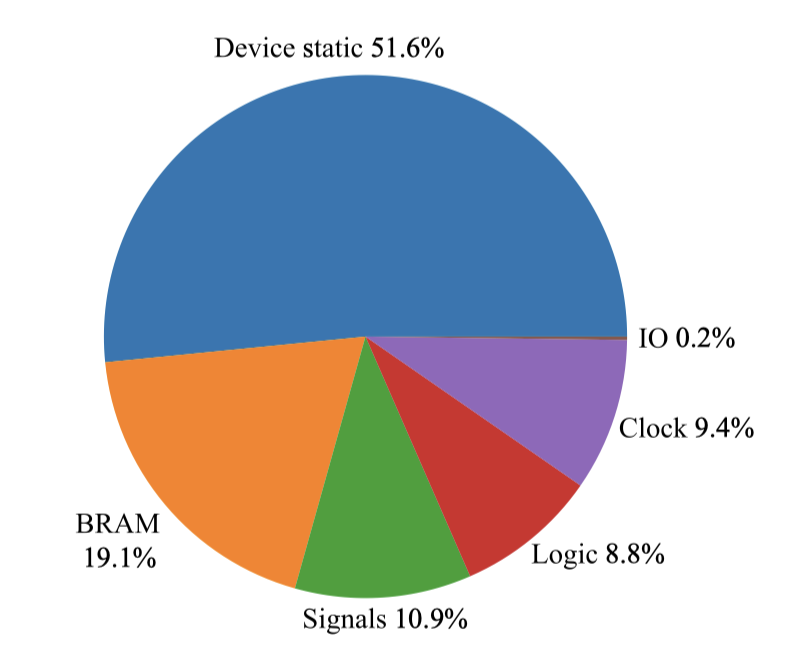
\includegraphics[width=0.8\textwidth]{../assets/Fig4.png}
% \end{center}
% \vspace{-0.1in}  
% \caption{Power consumption breakdown.}
% \label{fig:Power consumption breakdown.}
% \end{figure}

% \rule{\linewidth}{0.5pt}

\section{系统性能}

我们根据基准数据集的总体吞吐量(以每秒帧数为单位)和每秒处理的激活事件数来评估所提出的模块的性能。
为了测量处理时间,我们在测试平台中插入了一个硬件计数器。
当ARM处理器完成DDR3内存和建议模块的初始配置时,它开始计数,并在最终帧获得其分类结果时停止计数。
10 000 帧的处理时间为 62.1 秒,提供每秒 161 帧的帧速率。

对于激活事件的数量,我们使用 MATLAB 来模拟所提出模块的定点计算。 
使用此模拟器,激活事件的数量为 $4.2 \times 10^7$ 。
根据上述获取的处理时间,处理激活事件的性能为每秒 $6.72 \times 10^5$ 个事件。

为了使所提出的模块处理神经元的每个激活事件,需要更新其所有连续神经元的状态; 这需要从 DDR3 内存中获取 1024 个权重值。

鉴于所提出的模块运行在200 MHz并且数据总线宽度为64位,带宽可以高达1600 MB/s(权重在分类期间是只读的并且仅考虑一个方向)。
为了处理每个神经元激活事件,需要其所有连续神经元的权重。
由于我们为每个权重使用 16 位,并且每个神经元的最大扇出为 1024,因此数量应为 2 KB。
结合这两个约束,系统的最大性能为每秒 $8 \times 10^5$ 个事件。

将实际性能与理论值进行比较,带宽在所提出的设计中得到了很好的利用。
这些系统性能结果进一步表明外部存储器带宽是基于 FPGA 的 SNN 实现的瓶颈。
减少权重位宽和网络修剪等技术可以缓解这个问题; 特别是,网络剪枝已被证明在人工神经网络中是有效的。

% \section{Comparison with GPU}

% For comparison, the same SNN model is implemented with the PyTorch  framework to run on an NVIDIA Tesla P100 GPU.
% Note that GPUs are not suitable for event-driven updating, so we implement the timestepped updating algorithm instead.
% Again, we measure the execution time of the 10 000 frames of the MNIST test dataset.
% The runtime power during GPU execution is measured with the NVIDIA System Management Interface.

% The processing time on a GPU is 7.96 s and the average power consumption is 29.6 W.
% Therefore, although the proposed module demands more execution time, it consumes much less power than a GPU.
% This equates to much greater power efficiency: 337.6 frames per second per watt compared to 42.2 frames per second per watt on a GPU.
% These results imply that the proposed design is suitable for application scenarios that have strict constraints on power consumption and a tolerance for execution latency.

% \rule{\linewidth}{0.5pt}

\section{与GPU的比较}

为了进行比较,相同的 SNN 模型是使用 PyTorch 框架实现的,并在 NVIDIA Tesla P100 GPU上运行。
请注意,GPU 不适合事件驱动的更新,因此我们改为实现时间步进更新算法。 
我们再次测量 MNIST 测试数据集 10000 帧的执行时间。 
GPU 执行期间的运行时功率通过 NVIDIA 系统管理接口进行测量。

GPU 上的处理时间为 7.96 秒,平均功耗为 29.6 W。
因此,虽然所提出的模块需要更多的执行时间,但它的功耗比 GPU 少得多。 
这相当于更高的能效:每瓦每秒 337.6 帧,而 GPU 上每瓦每秒 42.2 帧。 
这些结果意味着所提出的设计适用于对功耗和执行延迟有严格限制的应用场景。
